%\documentclass[aspectratio=43]{beamer}
\documentclass[c]{beamer}
\usetheme{intridea}  %% Themenwahl

\usepackage[ngerman]{babel} 
\usepackage[T1]{fontenc}    % richtige Silbentrennung
\usepackage[utf8]{inputenc} % Umlaute etc.!
\usepackage{eurosym}
\usepackage{tikz}

\usetikzlibrary{arrows,decorations.pathmorphing,backgrounds,fit,positioning,shapes.symbols,chains}

%1

\title{Freifunk Hamburg}
\author{hamburg.freifunk.net}
\date{27. Juli 2013}


%2
\begin{document}
\maketitle

\begin{frame}{Was ist freifunk?}
	\begin{itemize}
		\item Initiative für freie, offene, kostenlose Funk- und Datennetzwerke
		\item freifunk steht jedem offen, als Nutzer oder Anbieter
		\item Als freifunk-Knoten (Zugangspunkt) dienen dafür vorbereitete WLAN-router
		\item In vielen Orten gibt es bereits Freifunknetze (Berlin, Wien, Augsburg, Lübeck, Kiel, Rheinland, Hamburg...)
	\end{itemize}
\end{frame}


%3
\begin{frame}{Was ist freifunk?}
	\textbf{Frei} wird verstanden als
	\begin{itemize}
		\item Öffentlich - jedem zugänglich
		\item Nicht kommerziell
		\item Im Besitz der Gemeinschaft
		\item Netzneutral - keine Manipulation der Datenströme
	\end{itemize}
	\textbf{Netzwerk} meint
	\begin{itemize}
		\item Kommunikation zwischen Menschen unter Verwendung digitaler Medien (Computer, Handys, Datennetze)
	\end{itemize}
\end{frame}


%4
\begin{frame}{Geschichte}
	\begin{itemize}
		\item OPAL-Netz in Berlin-Friedrichshain sorgte für Bedarf nach günstigen Breitbandverbindungen
		\item Linksys WRT54g --> Harald Welte gpl-violations.org --> OpenWRT (Jan. 2004)
		\item Entwicklung verschiedener meshing-Protokolle (OLSR, B.A.T.M.A.N., 802.11s...)
	\end{itemize}
	\begin{center}
		Die Kombination dieser drei Aspekte schafften Bedarf und Voraussetzungen für freifunk
	\end{center}
\end{frame}


%5
\begin{frame}{Mit freifunk ins Internet}
	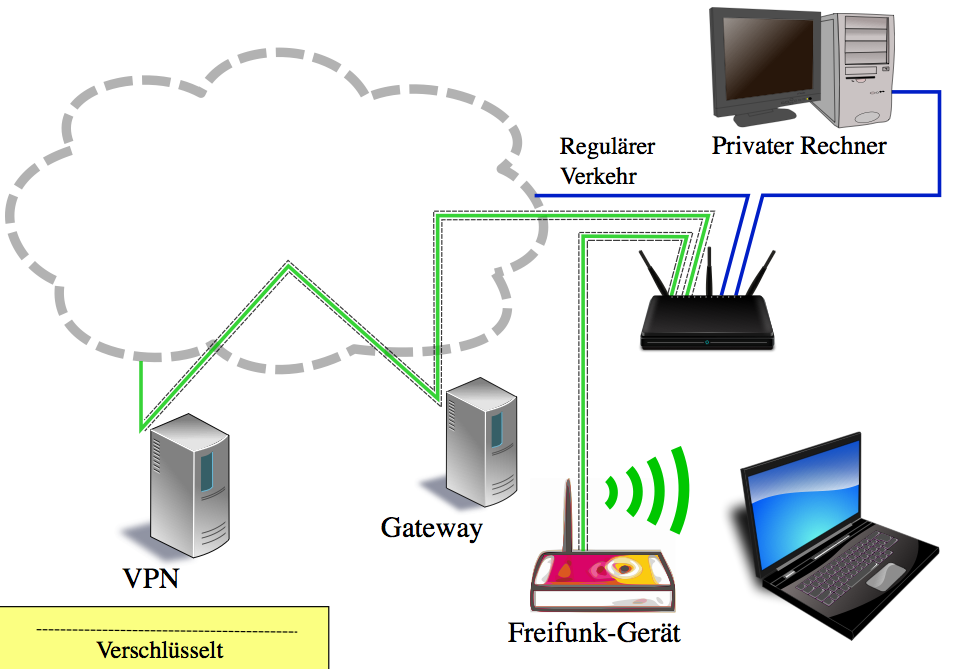
\includegraphics[height=180pt]{Bilder/Knotenanbindung2}
\end{frame}


%6
\begin{frame}{Ziel des Projekts}
	\begin{itemize}
		\item Verbreitung offener WLAN-Netzwerke
		\item Zugangshürden zum Internet minimieren
		\item Aufklärung und Sensibilisierung zum Thema "Kommunikations- und Informationsfreiheit''
		\item Menschen dazu befähigen, eigene Netze aufzubauen und zu betreiben
		\item Soziale Strukturen bilden und unterstützen
	\end{itemize}
\end{frame}


%7
\begin{frame}{Demo}
	\begin{itemize}
		\item Knotenkarte \href{http://knotenkarte.de}{http://knotenkarte.de}
	\end{itemize}
\end{frame}



%8
\begin{frame}{Warum WLAN?}
	\begin{itemize}
		\item Mit WLAN können Daten mobil mit hoher Bandbreite gesendet und empfangen werden
		\item Die Kosten für WLAN-Hardware sind gering und es entstehen kaum Betriebskosten (Router ab \EUR{15}, Strom ca. \EUR{10} im Jahr)
		\item WLAN kann auch dort eingesetzt werden, wo es keine Kabel gibt oder eine Kabelverbindung zu teuer ist
		%[Parks, Entwicklungsländer, etc...]
	\end{itemize}
\end{frame}


%9
\begin{frame}{Reichweite}
	\begin{center}
		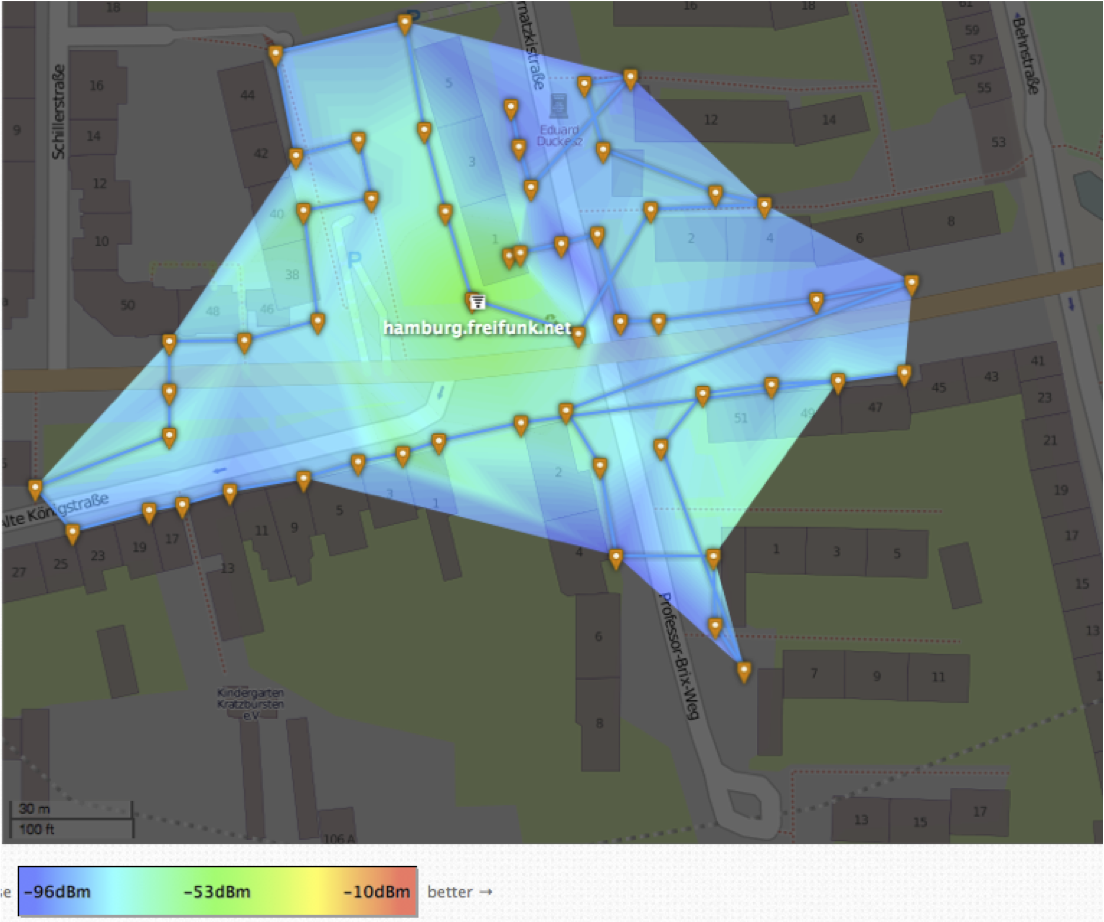
\includegraphics[height=180pt]{Reichweite_altona001}
	\end{center}
\end{frame}


%10
\begin{frame}{Mesh}
	Was ist ein mesh?
	\begin{itemize}
		\item to mesh = Englisch: vermaschen
		\item Selbst organisierende Netzwerke
		\item Jeder Router ist automatisch aktiver Teil des Netzwerks
		\item hamburg.freifunk.net Nutzt das Protokoll B.A.T.M.A.N.-adv.
	\end{itemize}
	Zwei SSIDs
	\begin{itemize}
		\item Freifunk Zugang: hamburg.freifunk.net
		\item Mashing (adhoc): f8:d1:11:87:52:2e
	\end{itemize}
\end{frame}


%11
\begin{frame}{Mesh}
	\begin{center}
		\begin{tikzpicture}
			\definecolor{outerCircleColour}{RGB}{220, 0, 103}
			\definecolor{innerCircleColour}{RGB}{255, 203, 18}
			\tikzstyle{vertex}=[circle, draw, color=outerCircleColour, ultra thick, minimum size=84pt]
			\tikzstyle{place}=[circle, draw, color=innerCircleColour, fill=innerCircleColour, minimum size=6pt, inner sep=0pt]

			\node [vertex] (a) {};
			\node [vertex, xshift=68pt, yshift=24pt] (b) {};
			\node [vertex, xshift=112pt, yshift=-20pt] (c) {};

			\node [place, label=above:$A$] (A) {};
			\node [place, xshift=68pt, yshift=24pt, label=above:$B$] (B) {};
			\node [place, xshift=112pt, yshift=-20pt, label=right:$C$] (C) {};

			\path[-, thick, color=gray]
			(A) edge (B)
			(B) edge (C);
		\end{tikzpicture}
	\end{center}
\end{frame}


%12
\begin{frame}{Mesh}
	\begin{center}
		\begin{tikzpicture}
\definecolor{outerCircleColour}{RGB}{220, 0, 103}
			\definecolor{innerCircleColour}{RGB}{255, 203, 18}
			\tikzstyle{vertex}=[circle, draw, color=outerCircleColour, ultra thick, minimum size=84pt]
			\tikzstyle{place}=[circle, draw, color=innerCircleColour, fill=innerCircleColour, minimum size=6pt, inner sep=0pt]

			\node [vertex] (a) {};
			\node [vertex, xshift=68pt, yshift=24pt] (b) {};
			\node [vertex, xshift=112pt, yshift=-20pt] (c) {};

			\node [place, label=above:$A$] (A) {};
			\node [place, xshift=68pt, yshift=24pt, label=above:$B$] (B) {};
			\node [place, xshift=112pt, yshift=-20pt, label=right:$C$] (C) {};

			\path[-, thick, color=gray]
			(A) edge (B)
			(B) edge (C)
			(A) edge[dashed] (C);
		\end{tikzpicture}
	\end{center}
\end{frame}

%13
\begin{frame}{Das Netz wächst}
	\begin{center}
		\begin{tikzpicture}
			\definecolor{outerCircleColour}{RGB}{220, 0, 103}
			\definecolor{innerCircleColour}{RGB}{255, 203, 18}
			\tikzstyle{vertex}=[circle, draw, color=outerCircleColour, ultra thick, minimum size=40pt]
			\tikzstyle{place}=[circle, draw, color=innerCircleColour, fill=innerCircleColour, minimum size=7pt, inner sep=0pt]

			\node [vertex] (a) {};
			\node [vertex, xshift=15pt, yshift=30pt] (b) {};
			\node [vertex, xshift=65pt, yshift=5pt] (c) {};
			\node [vertex, xshift=33pt, yshift=-3pt] (d) {};
			\node [vertex, xshift=85pt, yshift=-25pt] (e) {};
			\node [vertex, xshift=100pt, yshift=2pt] (f) {};
			\node [vertex, xshift=91pt, yshift=32pt] (g) {};
			\node [vertex, xshift=110pt, yshift=-52pt] (h) {};
			\node [vertex, xshift=124pt, yshift=23pt] (i) {};
			\node [vertex, xshift=134pt, yshift=-7pt] (j) {};
			\node [vertex, xshift=164pt, yshift=-14pt] (k) {};
			\node [vertex, xshift=144pt, yshift=-66pt] (l) {};
			\node [vertex, xshift=170pt, yshift=-46pt] (m) {};
			\node [vertex, xshift=201pt, yshift=-59pt] (n) {};

			\node [place] (A) {};
			\node [place, xshift=15pt, yshift=30pt] (B) {};
			\node [place, xshift=65pt, yshift=5pt] (C) {};
			\node [place, xshift=33pt, yshift=-3pt] (D) {};
			\node [place, xshift=85pt, yshift=-25pt] (E) {};
			\node [place, xshift=100pt, yshift=2pt] (F) {};
			\node [place, xshift=91pt, yshift=32pt] (G) {};
			\node [place, xshift=110pt, yshift=-52pt] (H) {};
			\node [place, xshift=124pt, yshift=23pt] (I) {};
			\node [place, xshift=134pt, yshift=-7pt] (J) {};
			\node [place, xshift=164pt, yshift=-14pt] (K) {};
			\node [place, xshift=144pt, yshift=-66pt] (L) {};
			\node [place, xshift=170pt, yshift=-46pt] (M) {};
			\node [place, xshift=201pt, yshift=-59pt] (N) {};

			\path[-, thick, color=gray]
			(A) edge (B)
			(A) edge (D)
			(B) edge (D)
			(C) edge (D)
			(C) edge (E)
			(C) edge (F)
			(C) edge (G)
			(E) edge (F)
			(E) edge (H)
			(F) edge (G)
			(F) edge (I)
			(F) edge (J)
			(G) edge (I)
			(H) edge (L)
			(I) edge (J)
			(J) edge (K)
			(K) edge (M)
			(L) edge (M)
			(M) edge (N);
		\end{tikzpicture}
	\end{center}
\end{frame}


%14
\begin{frame}{Netzwerke verbinden sich untereinander}
	\begin{columns}[c]
		\begin{column}[l]{.4\textwidth}
			\scalebox{0.6}[0.6]{
			\begin{tikzpicture}
				\definecolor{outerCircleColour}{RGB}{220, 0, 103}
				\definecolor{innerCircleColour}{RGB}{255, 203, 18}
				\tikzstyle{vertex}=[circle, draw, color=outerCircleColour, ultra thick, minimum size=40pt]
				\tikzstyle{place}=[circle, draw, color=innerCircleColour, fill=innerCircleColour, minimum size=7pt, inner sep=0pt]

				\node [vertex] (a) {};
				\node [vertex, xshift=15pt, yshift=30pt] (b) {};
				\node [vertex, xshift=65pt, yshift=5pt] (c) {};
				\node [vertex, xshift=33pt, yshift=-3pt] (d) {};
				\node [vertex, xshift=85pt, yshift=-25pt] (e) {};
				\node [vertex, xshift=100pt, yshift=2pt] (f) {};
				\node [vertex, xshift=91pt, yshift=32pt] (g) {};
				\node [vertex, xshift=110pt, yshift=-52pt] (h) {};
				\node [vertex, xshift=124pt, yshift=23pt] (i) {};
				\node [vertex, xshift=134pt, yshift=-7pt] (j) {};
				\node [vertex, xshift=164pt, yshift=-14pt] (k) {};
				\node [vertex, xshift=144pt, yshift=-66pt] (l) {};
				\node [vertex, xshift=170pt, yshift=-46pt] (m) {};
				\node [vertex, xshift=201pt, yshift=-59pt] (n) {};

				\node [place] (A) {};
				\node [place, xshift=15pt, yshift=30pt] (B) {};
				\node [place, xshift=65pt, yshift=5pt] (C) {};
				\node [place, xshift=33pt, yshift=-3pt] (D) {};
				\node [place, xshift=85pt, yshift=-25pt] (E) {};
				\node [place, xshift=100pt, yshift=2pt] (F) {};
				\node [place, xshift=91pt, yshift=32pt] (G) {};
				\node [place, xshift=110pt, yshift=-52pt] (H) {};
				\node [place, xshift=124pt, yshift=23pt] (I) {};
				\node [place, xshift=134pt, yshift=-7pt] (J) {};
				\node [place, xshift=164pt, yshift=-14pt] (K) {};
				\node [place, xshift=144pt, yshift=-66pt] (L) {};
				\node [place, xshift=170pt, yshift=-46pt] (M) {};
				\node [place, xshift=201pt, yshift=-59pt] (N) {};

				\path[-, thick, color=gray]
				(A) edge (B)
				(A) edge (D)
				(B) edge (D)
				(C) edge (D)
				(C) edge (E)
				(C) edge (F)
				(C) edge (G)
				(E) edge (F)
				(E) edge (H)
				(F) edge (G)
				(F) edge (I)
				(F) edge (J)
				(G) edge (I)
				(H) edge (L)
				(I) edge (J)
				(J) edge (K)
				(K) edge (M)
				(L) edge (M)
				(M) edge (N);
			\end{tikzpicture}}
		\end{column}
		\begin{column}{0.185\textwidth}
			\begin{uncoverenv}<2->
				\begin{tikzpicture}
					\definecolor{outerCircleColour}{RGB}{220, 0, 103}
					\definecolor{innerCircleColour}{RGB}{255, 203, 18}

					\draw[color=white] (280pt, 85pt) arc (0:0:0pt);
					\draw[color=white] (-180pt, 85pt) arc (0:0:0pt);

					\draw[color=outerCircleColour, thick, xshift=-50pt, yshift=9pt] (-110pt, 0pt) arc (270:450:6pt);
					\draw[color=outerCircleColour, thick, xshift=-50pt, yshift=11pt] (-110pt, 0pt) arc (270:450:4pt);
					\draw[color=outerCircleColour, thick, xshift=-50pt, yshift=13pt] (-110pt, 0pt) arc (270:450:2pt);

					\draw[color=outerCircleColour, thick, xshift=-9pt, yshift=21pt] (-110pt, 0pt) arc (90:270:6pt);
					\draw[color=outerCircleColour, thick, xshift=-9pt, yshift=19pt] (-110pt, 0pt) arc (90:270:4pt);
					\draw[color=outerCircleColour, thick, xshift=-9pt, yshift=17pt] (-110pt, 0pt) arc (90:270:2pt);

					\draw[color=gray, ultra thick, xshift=-50pt, yshift=15] (-103pt, 0pt) edge[dashed] (-74pt, 0pt);
				\end{tikzpicture}
			\end{uncoverenv}
		\end{column}
		\begin{column}[r]{.5\textwidth}
			\reflectbox{
			\scalebox{0.6}[0.6]{
			\begin{tikzpicture}
				\definecolor{outerCircleColour}{RGB}{220, 0, 103}
				\definecolor{innerCircleColour}{RGB}{255, 203, 18}
				\tikzstyle{vertex}=[circle, draw, color=outerCircleColour, ultra thick, minimum size=40pt]
				\tikzstyle{place}=[circle, draw, color=innerCircleColour, fill=innerCircleColour, minimum size=7pt, inner sep=0pt]

				\node [vertex] (a) {};
				\node [vertex, xshift=15pt, yshift=30pt] (b) {};
				\node [vertex, xshift=65pt, yshift=5pt] (c) {};
				\node [vertex, xshift=33pt, yshift=-3pt] (d) {};
				\node [vertex, xshift=85pt, yshift=-25pt] (e) {};
				\node [vertex, xshift=100pt, yshift=2pt] (f) {};
				\node [vertex, xshift=91pt, yshift=32pt] (g) {};
				\node [vertex, xshift=110pt, yshift=-52pt] (h) {};
				\node [vertex, xshift=124pt, yshift=23pt] (i) {};
				\node [vertex, xshift=134pt, yshift=-7pt] (j) {};
				\node [vertex, xshift=164pt, yshift=-14pt] (k) {};
				\node [vertex, xshift=144pt, yshift=-66pt] (l) {};
				\node [vertex, xshift=170pt, yshift=-46pt] (m) {};
				\node [vertex, xshift=201pt, yshift=-59pt] (n) {};

				\node [place] (A) {};
				\node [place, xshift=15pt, yshift=30pt] (B) {};
				\node [place, xshift=65pt, yshift=5pt] (C) {};
				\node [place, xshift=33pt, yshift=-3pt] (D) {};
				\node [place, xshift=85pt, yshift=-25pt] (E) {};
				\node [place, xshift=100pt, yshift=2pt] (F) {};
				\node [place, xshift=91pt, yshift=32pt] (G) {};
				\node [place, xshift=110pt, yshift=-52pt] (H) {};
				\node [place, xshift=124pt, yshift=23pt] (I) {};
				\node [place, xshift=134pt, yshift=-7pt] (J) {};
				\node [place, xshift=164pt, yshift=-14pt] (K) {};
				\node [place, xshift=144pt, yshift=-66pt] (L) {};
				\node [place, xshift=170pt, yshift=-46pt] (M) {};
				\node [place, xshift=201pt, yshift=-59pt] (N) {};

				\path[-, thick, color=gray]
				(A) edge (B)
				(A) edge (D)
				(B) edge (D)
				(C) edge (D)
				(C) edge (E)
				(C) edge (F)
				(C) edge (G)
				(E) edge (F)
				(E) edge (H)
				(F) edge (G)
				(F) edge (I)
				(F) edge (J)
				(G) edge (I)
				(H) edge (L)
				(I) edge (J)
				(J) edge (K)
				(K) edge (M)
				(L) edge (M)
				(M) edge (N);
			\end{tikzpicture}}}
		\end{column}
	\end{columns}
\end{frame}


%15
\begin{frame}{Ein Beispiel in Wilhelmsburg}
	\begin{center}
		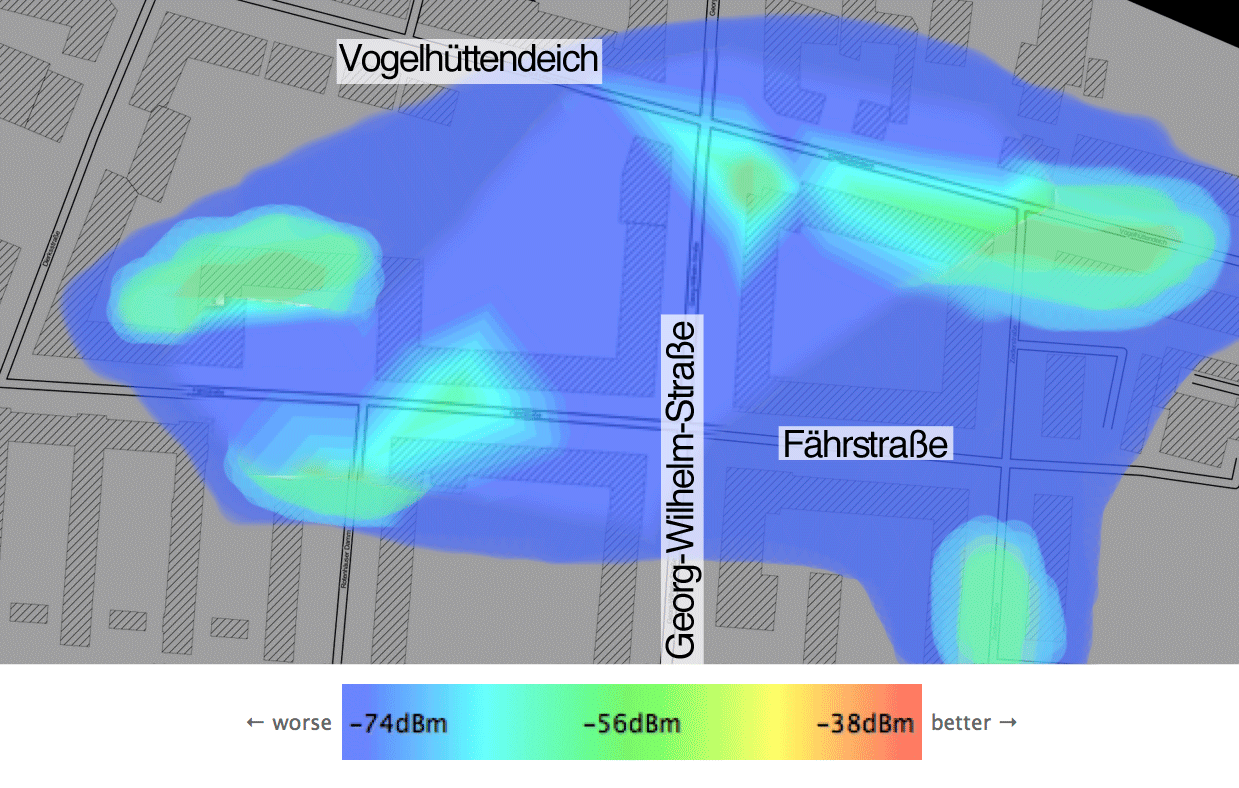
\includegraphics[width=0.9\textwidth]{wilhelmsburg}
	\end{center}
\end{frame}


%16
\begin{frame}{Sicherheit}
	\begin{itemize}
		\item Da freifunk kein Kennwort nutzt, ist die Funkstrecke zum Zugangspunkt (wie bei allen offenen WLANs) unverschlüsselt
		\item Je nach Relevanz, empfiehlt es sich nach Möglichkeit verschlüsselte Protokolle zu nutzen (https://, ftps://, ssh, ggf. eigenes VPN) zu nutzen – wie sonst auch im Netz
		\item Verbindungen über die gateways sind verschlüsselt (fastd) --> kein Zugriff auf das „Heimnetzwerk“ möglich
	\end{itemize}
\end{frame}


%17
\begin{frame}{Störerhaftung}
	\begin{itemize}
		\item Die Zugangspunkte gehen nicht direkt in das Internet
		\item Es wird über das Internet eine mit fastd verschlüsselte VPN Verbindung zu den gateways aufgebaut
		\item Selbst die gateways sind nicht die Ausgänge ins GBI, sondern bauen wiederum VPNs ins Ausland auf
	\end{itemize}
	Resultat:
	\begin{itemize}
		\item \begin{it}Vorteil\end{it}: Störerhaftung nicht durchsetzbar
		\item \begin{it}Nachteil\end{it}: Bandbreiten-limitierung durch Verschlüsselung (auf den kleinen routern ca. 6Mb/s)
	\end{itemize}
\end{frame}


%18
\begin{frame}{Community Agreement}
	\begin{itemize}
		\item Sei Fair!
		\item Achte auf deine Sicherheit!
		\item Keine rechtswidrige Nutzung!
	\end{itemize}
\end{frame}

%19
\begin{frame}{Geräte}
	\begin{columns}[c]
		\begin{column}{0.5\textwidth}
			\begin{itemize}
				\item TP-Link 741nd (ab \EUR{15})
				\item TP-Link 841nd
				\item TP-Link 842nd (ab \EUR{25})
				\begin{itemize}
					\item Atheros AR7241 SOC
					\item 8 MB flash	
					\item 32MB RAM
					\item 300Mbit/s
				\end{itemize}
				\item TP-Link 1043nd
				\item TP-Link 3600
			\end{itemize}
		\end{column}
		\begin{column}{0.5\textwidth}
			\begin{center}
				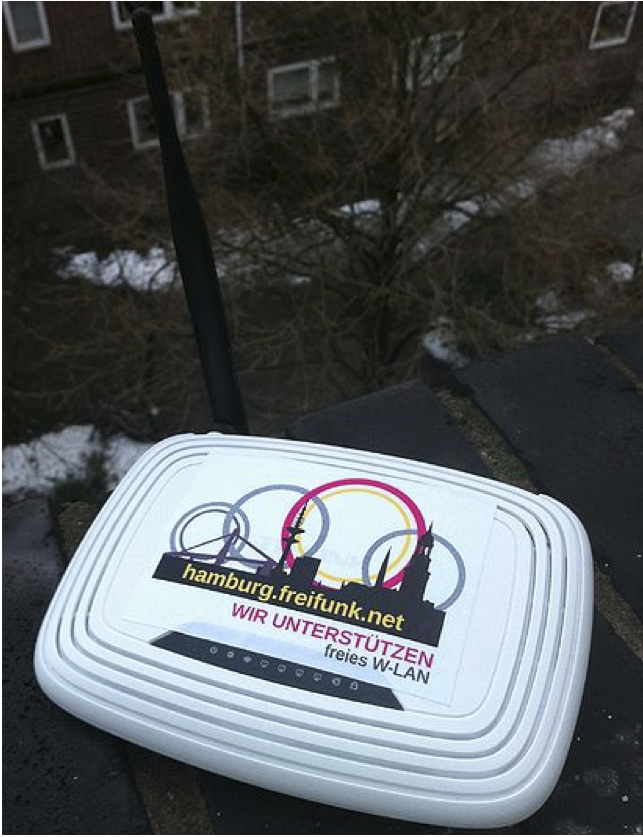
\includegraphics[height=150pt]{741nd}
			\end{center}
		\end{column}
	\end{columns}
\end{frame}


%20
\begin{frame}{Dienste}
	Implementiert
	\begin{itemize}
		\item Internet
		\item Stadtweites Intranet (IPv4 \& IPv6)
	\end{itemize}
	Teilweise implementiert
	\begin{itemize}
		\item IC-VPN, Chaos-VPN, DN42... 
	\end{itemize}
	Noch zu implementieren
	\begin{itemize}
		\item Voice over IP (SIP)
		\item DNS (für das Intranet)
		\item Alles was du anbieten möchtest...
	\end{itemize}
\end{frame}


%21
\begin{frame}{Ausblick}
	\begin{itemize}
		\item Weitere gateways
		\item Wachsende Zahl von Zugangspunkten in Cafés, Restaurants, etc.
		\item Kooperation mit der Stadt Hamburg (WLAN in Parks, Tourismus-Förderung...)
		\item Kooperation mit dem HVV
		\item Hochschulen / Studentenwerk
		\item ...
	\end{itemize}
\end{frame}


%22
\begin{frame}{Projekte}
	\begin{itemize}
		\item Antennenbau-Workshop
		\item Outdoor-Gehäuse
		\item Solarbetrieb
		\item Flash-Workshops
		\item PPPoE implementieren
		\item Privates WLAN implementieren
		\item Internet Uplink über WLAN
		\item Vernwartung und Monitoring der Knoten
		\item Mailserver aufsetzen
		\item Knoteneinstellungsverwaltung über's Netz
		\item ...
	\end{itemize}
\end{frame}


%23
\begin{frame}{Wie kann man mitmachen?}
	\begin{itemize}
		\item Alle können Freifunker/innen werden, besondere technische Kenntnisse sind nicht notwendig
		\item Werde ein Teil des Netzwerks, indem du bei dir im Haus einen Freifunk-Knoten aufstellst
		\item Treffen jeden Montag um 19:00 Uhr in den Räumen des CCCHH
		\item Verbreite die Idee!
	\end{itemize}
\end{frame}


%24
\begin{frame}{Vielen Dank!}
	\begin{columns}
		\begin{column}{0.6\textwidth}
			\begin{itemize}
				\item Netz: hamburg.freifunk.net
				\item Mail: kontakt@hamburg.freifunk.net
		\end{itemize}
		\end{column}
		\begin{column}{0.5\textwidth}
			\begin{center}
				
\includegraphics[width=0.5\textwidth]{cc-by}
			\end{center}
		\end{column}
	\end{columns}
\end{frame}

\end{document}